\chapter{Analyse des principaux sites web}
\section{Objectif de l'analyse}
Le but de l'analyse est de parcourir les sites les plus visités au monde d'après le classement Alexa \footnote{Alexa \cite{AlexaTop} est une entreprise qui appartient à Amazon et qui est principalement connue pour les statistiques qu'elle fournit sur le trafic Web dans le monde entier.}. Ensuite, déterminer s'ils contiennent des trackers et, le cas échéant, leur nature. Deux types d'expérience peuvent être menés :
\begin{enumerate}
	\item Le premier consiste en une analyse à long terme.
	\item Le second consiste en une analyse ponctuelle.
\end{enumerate}

Le premier type d'expérience a pour but de déterminer si les sites modifient leurs trackers au fil du temps.
Le second type permet d'avoir une image globale du niveau de traçage opéré par les principaux sites à un instant donné. Il donne également la possibilité de tester l'efficacité des extensions de navigateur qui affirment protéger la vie privée (voir \autoref{results_plugins}).

\section{Description de l'outil implémenté}
L'idée initiale était d'utiliser le framework \textit{fpdetective} \cite{Acar:2013:FDW:2508859.2516674}. C'est un framework conçu pour la détection et l'analyse d'outils (\textit{fingerprinters}, voir \autoref{fingerprinters}) qui créent des empreintes de navigateurs. Ce framework semblait prometteur mais son efficacité s'est révélée insuffisante et il ne fonctionnait pas correctement. En effet, aucun \textit{fingerprinter} n'était détecté alors que certains étaient manifestement présents sur plusieurs sites web visités.

Étant donné que \textit{fpdetective} ne pouvait fournir les résultats demandés, la création d'un outil dédié à cette tâche était nécessaire. De plus, cela permettait davantage de souplesse au niveau des décisions d'implémentation et du paramétrage de la recherche de trackers.
\newline

L'outil a été implémenté en Java. Il se compose de deux éléments : le \textit{crawler} qui visite les sites web et exporte leur contenu au format HTTP Archive (HAR) et le \textit{parser} qui traite les fichiers HAR en déterminant si les sites correspondants renferment des trackers.
L'outil a été développé sous Eclipse et est destiné à être utilisé sur Linux. Un exécutable JAR est également disponible.
La liste des options disponibles au lancement de l'outil est détaillé dans l'Annexe \ref{options_outil_implémenté}.
\newline

\subsection{Crawler}
\label{crawler}
\subsubsection{Choix d'implémentation}
Afin d'automatiser le navigateur et de parcourir les sites sans intervention humaine, \textit{Selenium} \footnote {\textit{Selenium} \cite{selenium_homepage} est une suite d'outils qui permet d'automatiser les navigateurs. On peut par exemple créer des scripts qui vont faire visiter un navigateur sur différents sites et effectuer plusieurs actions.} est utilisé dans le \textit{crawler} ou plus précisément, le pilote \textit{FirefoxDriver} de \textit{Selenium}. Il permet de lancer une instance de Firefox et d'interagir avec celle-ci.

La première implémentation traitait directement le code source de la page. Il était possible d'aller sur le moteur de recherche Google, de sélectionner le champ de recherche, de taper une requête et de récupérer le résultat. Cependant, le processus était assez lent et incomplet car on ne pouvait pas récupérer les requêtes et les réponses HTTP. On pouvait juste collecter les éléments associés à des balises (par exemple, récupérer toutes les images via les balises de type \textit{<img>}, les scripts avec les balises \textit{<script>},...) mais tout n'était pas récupérable car certains éléments étaient chargés sans être identifiés.

Afin de pallier à ce problème, la deuxième implémentation utilisait un proxy \footnote{Un proxy est un serveur qui sert d'intermédiaire afin d'accéder à un réseau et récupérer des ressources d'un autre serveur.} qui exportait le contenu du site au format HTTP Archive \footnote{HTTP Archive est un format ouvert qui permet d'exporter des échanges de données collectés par un outil de monitoring HTTP \cite{har_spec}.}. L'ensemble des requêtes et réponses HTTP était récupéré et enregistré dans un fichier. Le parcours du code source de la page (qui donnait des résultats finalement incomplets) a été supprimé afin de rendre le programme plus rapide. Cette fois, le problème était que le proxy n'exécutait pas le JavaScript. Il en résultait que de nombreux sites ne pouvaient être chargés correctement (cela pouvait varier de 15 à 30\% d'échecs) et il était alors impossible de les traiter.

La troisième solution, qui est la dernière implémentée, consiste à utiliser le pilote \textit{FirefoxDriver} pour charger automatiquement les sites, sans parcours du code source ni utilisation de proxy. Le contenu des sites est exporté au format HTTP Archive à l'aide de deux extensions qui ont été installées dans Firefox.
\begin{itemize}
	\item La première, Firebug \cite{firebug_homepage}, est une extension utilisée principalement par les développeurs de sites web afin de les débugger. Elle permet de monitorer les éléments d'une page (CSS, HTML, JavaScript) en direct.
	\item La seconde, NetExport \cite{netexport_homepage}, est une extension de Firebug qui permet d'exporter toutes les données d'une page au format HTTP Archive de façon automatique moyennant un paramétrage adéquat.
\end{itemize}

Le taux de réussite de l'export des données des sites s'est grandement amélioré. Néanmoins, certains sites ne sont toujours pas chargés correctement.
Une hypothèse est que certains sites sont hébergés sur des serveurs lointains et leurs éléments prennent alors plus de temps à charger. Ainsi, lorsque ces sites contiennent une grande quantité d'éléments, le pilote renvoie une exception de type \textit{timeout} et le chargement du site est finalement en échec.

Afin de vérifier cette hypothèse, une série de tests a été mise en place. Le test consistait à faire varier la valeur du timeout et de vérifier si cela influençait le nombre de sites en échec avec le \textit{crawler}. Celui-ci a donc été lancé sur le TOP 500 avec des valeurs de timeout différentes.
Le graphique est visible à la \autoref{graphique_timeout} et il montre que cette hypothèse est vérifiée.
\newline

\begin{figure}[!h]
	\centering
	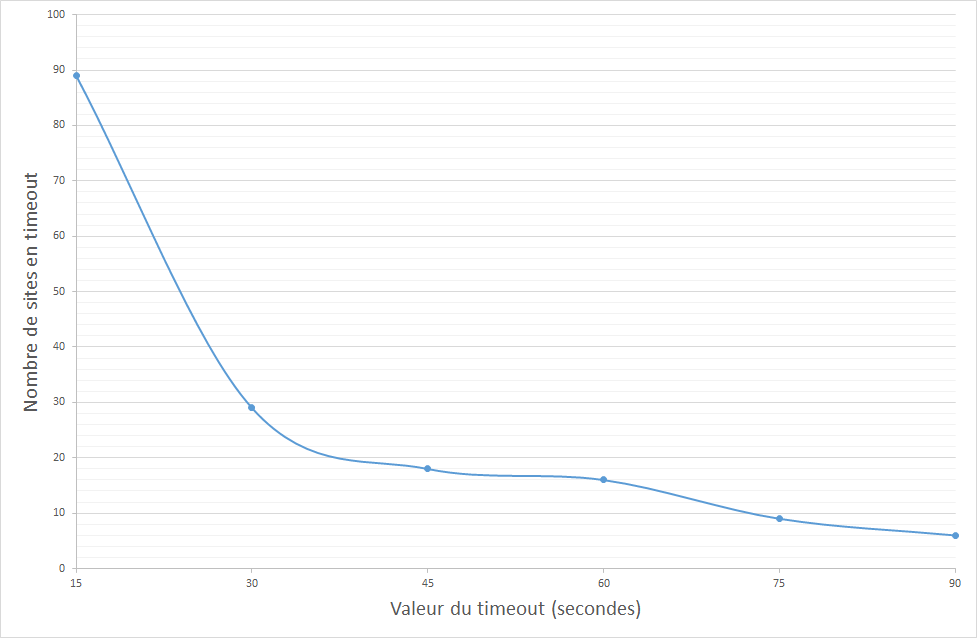
\includegraphics[scale=.6]{timeouts/Timeouts.png}
	\caption{\label{graphique_timeout}Nombre de sites en échec en fonction du timeout sur le TOP 500.}
\end{figure}

Une amélioration a été apportée à l'outil afin de compter le nombre de cookies Flash créés lors de chaque visite de site. Cette fonctionnalité a été implémentée au sein du \textit{crawler} étant donné que ce n'est pas possible d'accéder à cette information avec l'aide des fichiers HTTP Archive analysés par le \textit{parser}. Cela signifie qu'une partie des résultats est déjà disponible lorsque le \textit{crawler} a fini de visiter les sites.

A son lancement, il supprime l'ensemble des cookies Flash (les fichiers .sol) dans le dossier \textit{.macromedia/Flash\_Player/\#SharedObjects/XXXXXXXX/}. Il supprime également les cookies Firefox en se connectant à la base de données SQLite dans \textit{.mozilla/firefox/<profil>/cookies.sqlite} et en vidant la table \textit{moz\_cookies}. Cela permet de s'assurer que la visite des sites ne sera pas influencée par la présence de cookies antérieurs.

\subsubsection{Changements opérés sur les extensions}
\label{changements_extensions}
Deux modifications ont été nécessaires sur l'extension \textit{NetExport} de \textit{Firebug}. Les changements dans leur code source sont détaillés dans l'Annexe \ref{modifications_extensions}.

La première concerne la génération des fichiers HTTP Archive. Par défaut, l'extension ajoute un champ qui n'est pas standard par rapport à la spécification du format HAR \cite{har_spec}. Il en résulte que les fichiers peuvent alors être considérés comme corrompus alors que la présence ou non de ce champ n'influence en rien les résultats qui nous concernent. La génération de ce champ a donc été supprimée dans le fichier \textit{/chrome/content/netexport/harBuilder.js} de \textit{NetExport}.

La seconde modification concerne le nom des fichiers générés. Par défaut, l'extension ajoute la date à l'URL du site dans les noms de fichier. Cela pose des difficultés supplémentaires au \textit{parser} lors de la récupération et du traitement de ces fichiers (voir \autoref{parser}). L'extension a donc été modifiée afin de n'utiliser que l'URL du site dans les noms du fichier. Cette modification a été effectuée dans le fichier \textit{/chrome/content/netexport/automation.js}. Sur Linux, lorsqu'un fichier de même nom existe déjà, un tiret suivi du numéro de copie est ajouté au nom de fichier avant son extension.

\subsubsection{Fonctionnement}
Le \textit{crawler} fonctionne de la manière suivante. D'abord, il vérifie que le répertoire donné en argument est accessible en écriture et il crée deux dossiers nommés "logs" et "results" qui sont destinés à contenir respectivement les logs et les résultats du \textit{crawler}. Ensuite, le fichier de log (log\_crawler.txt) est créé, le dossier des cookies Flash est détecté (s'il y en a plusieurs, l'utilisateur est invité à indiquer le bon dossier) et la base de données SQLite des cookies Firefox est vidée (le dossier des paramètres de l'utilisateur est automatiquement trouvé grâce au profil Firefox spécifié en argument au lancement du programme). La liste des sites à visiter est ainsi chargée depuis le fichier spécifié et en fonction de l'intervalle donné par l'utilisateur. Puis, le profil Firefox choisi est chargé et différents paramètres de configuration des extensions sont également réglés avant que le pilote ne soit initialisé et qu'il lance Firefox. Après le lancement du pilote, un délai de 5 secondes laisse le temps à Firefox de se lancer et de charger ses extensions.
\newline

Après cette phase de préparation, le parcours des sites commence. Le pilote dirige Firefox sur l'URL du premier site de la liste. Lorsque le chargement de la page est terminé, un délai de 8 secondes permet aux extensions d'enregistrer le fichier HTTP Archive. Le nombre de cookies Flash est enregistré pour chaque site.

Si la page s'est chargée avant la limite de timeout définie par l'utilisateur (par défaut, 30 secondes), l'enregistrement est considéré comme valide et le pilote charge le site suivant dans la liste.

Si un site fait un timeout et que l'utilisateur a précisé un nombre de tentatives supérieur à 1, le pilote dirige Firefox sur la page "about:blank" (cela permet d'éviter des problèmes d'écriture de fichiers avec les extensions) puis le redirige sur le site pour un nouvel essai. Ce processus est répété à chaque timeout jusqu'à atteindre le nombre maximal de tentatives. Si le site fait encore un timeout lors de la dernière tentative, il est alors considéré en échec et son URL est inscrite dans une liste reprenant tous les sites en échec. A la deuxième tentative, l'URL du site a déjà été enregistrée dans une autre liste reprenant tous les sites ayant fait un timeout, cela permet de garder une trace des sites dont la visite a rencontré un problème mais qui ont finalement pu être chargés. 

Il arrive également qu'un site ne puisse tout simplement pas être chargé (à cause d'une erreur dans son code source par exemple). Son URL est alors directement enregistrée dans la liste reprenant les sites en échec.
\newline
\newpage

Lorsque le parcours de l'ensemble des sites est terminé, le programme efface les fichiers inutiles générés lors de la visite des pages "about:blank" et détaille l'ensemble des sites ayant subi au moins un timeout et les sites en échec. La liste des sites avec leur nombre de cookies Flash est enregistrée en ordre décroissant dans le fichier "stats\_flash-cookies.csv" du dossier "logs". Pour terminer, le pilote est arrêté (ce qui entraîne la fermeture de Firefox) et le fichier de log est fermé.
\newline

Il a été nécessaire d'implémenter une fonctionnalité qui redémarre Firefox à intervalles réguliers. En effet, certains sites ouvrent des pop-ups et si le navigateur n'est pas fermé, ces derniers s'accumulent et occupent une part plus importante de ressources. Le redémarrage du navigateur permet de fermer toutes ces fenêtres ouvertes de façon intempestive afin de garantir une meilleure stabilité du \textit{crawler}.

\subsection{Parser}
\label{parser}
\subsubsection{Choix d'implémentation}
Lors de la visite des sites par le \textit{crawler}, il arrive que celui-ci doive refaire de nouvelles visites afin d'exporter correctement le fichier HTTP Archive d'un site. Il en résulte que plusieurs fichiers pour le même site soient disponibles. Par exemple, on peut très bien voir des fichiers tels que \textit{monsite.com.har}, \textit{monsite.com-1.har}, etc. Lors de l'analyse de ces fichiers par le \textit{parser}, celui-ci considère seulement la dernière version du fichier comme étant valide. Il ignore donc les autres fichiers concernant le même site (si jamais il y en a plusieurs) car ils sont généralement corrompus ou incomplets.
\newline

Lors de l'analyse d'un fichier, l'URL du site est extraite (c'est le nom du fichier) et l'autorité en charge pour son domaine est automatiquement récupérée via une requête DNS de type SOA. Cela permettra de déterminer si une URL présente dans le site appartient au même domaine ou si elle provient d'un domaine différent.

Si l'autorité du domaine du site analysé ne peut être récupérée, l'analyse du site est considérée comme étant en échec et le nom du fichier en cours d'analyse est ajouté dans une liste reprenant tous les fichiers en échec.

Si l'autorité du domaine d'une URL analysée au sein d'un fichier ne peut être récupérée, l'analyse de cette URL est passée mais l'analyse des URL suivantes du fichier continue. Un message est imprimé dans le log pour préciser que la récupération de l'autorité du domaine de l'URL n'a pas pu être récupérée.

Lorsqu'une URL est constituée d'une adresse IP, l'outil fait une requête DNS afin de connaître le nom associé à cette IP. S'il n'y parvient pas, l'analyse de l'URL est passée mais le processus d'analyse continue comme c'est le cas lorsqu'une autorité ne peut être récupérée pour une URL. Ceci est dû au fait que la libraire utilisée (\textit{dnsjava}) pour effectuer les requêtes DNS n'est pas en mesure d'effectuer des requêtes SOA pour des adresses IP.
\newline

Le fonctionnement de la récupération de l'autorité d'une URL est le suivant : tout d'abord, la requête est effectuée sur l'hôte de l'URL. Si aucune réponse n'est retournée, la requête est effectuée sur le domaine parent et ainsi de suite, jusqu'à trouver une réponse ou arriver au domaine le plus haut (voir \autoref{dns_soa}).

Un système de mise en cache a été mis en place afin de limiter le nombre de requêtes effectuées et d'améliorer la rapidité d'accès à l'information.

\begin{figure}[h]
	\centering
	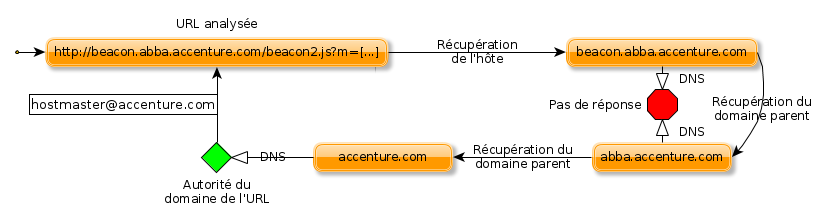
\includegraphics[scale=0.55]{figures/DNS_SOA.png}
	\caption{\label{dns_soa}Schéma de récupération de l'autorité du domaine.}
\end{figure}

\subsubsection{Limitation des requêtes DNS de type SOA}
Le recours aux informations SOA permet généralement de déterminer si deux sites appartiennent au même domaine. C'est ainsi que lors de la visite de \textit{youtube.com}, les images provenant de \textit{ytimg.com} ne sont pas détectées comme provenant d'un site externe. %(voir \autoref{dig_youtube} et \autoref{dig_ytimg}).
En effet, si on effectue deux requêtes DNS de type SOA pour \textit{youtube.com} et \textit{ytimg.com}, la même autorité de domaine est renvoyée : \textit{dns-admin@google.com}.
Dans ce cas, toute URL présente dans le site \textit{youtube.com} provenant de \textit{ytimg.com} ne sera pas considérée comme extérieure au site.
\newline

%\begin{figure}[h]
%	\centering
%	\lstinputlisting[style=dig]{examples/dig_youtube.com}
%	\caption{\label{dig_youtube}Informations SOA pour \textit{youtube.com}}.
%\end{figure}

%\begin{figure}[h]
%	\centering
%	\lstinputlisting[style=dig]{examples/dig_ytimg.com}
%	\caption{\label{dig_ytimg}Informations SOA pour \textit{ytimg.com}}.
%\end{figure}
%Comme vous pouvez le voir, les sites \textit{youtube.com} et \textit{ytimg.com} sont sous la même autorité qui est \textit{dns-admin@google.com}. 


Cependant, il peut y avoir des faux positifs résultant des réponses reçues. Lors des analyses, un phénomène a été remarqué: à certains moments, la requête DNS peut renvoyer une réponse différente. Ceci a été observé pour le domaine \textit{p8.qhimg.com}. %(voir \autoref{dig_p8.qhimg.com_1}%% et \autoref{dig_p8.qhimg.com_2}).
Dans ce cas précis, la requête DNS précise que l'autorité du site est en fait celle de l'hébergeur de contenu \textit{cloudfront.net} (qui est lui-même hébergé sur les serveurs d'\textit{Amazon}) et non plus celle du site visité. Afin d'éviter ce problème, il serait possible d'utiliser une liste des différentes autorités mise à jour en dehors du programme et vérifiée de façon indépendante et périodique. Cela n'a pas été jugé nécessaire lors de l'implémentation car le problème survient assez rarement (lors du lancement du \textit{parser} sur l'analyse de 1000 sites, cette situation s'est produite à seulement 2 reprises).

%\begin{figure}[h]
%	\centering
%	\lstinputlisting[style=dig]{examples/dig_p8.qhimg.com_1}
%	\caption{\label{dig_p8.qhimg.com_1}Informations SOA pour \textit{p8.qhimg.com}}.
%\end{figure}

%\begin{figure}[h]
%	\centering
%	\lstinputlisting[style=dig]{examples/dig_p8.qhimg.com_2}
%	\caption{\label{dig_p8.qhimg.com_2}Informations SOA pour \textit{p8.qhimg.com}, 10 secondes plus tard}.
%\end{figure}

\subsubsection{Critères qualifiant un tracker}
Le \textit{parser} parcourt l'ensemble des requêtes et réponses HTTP effectuées lors du chargement du site. Afin de déterminer si une ressource chargée est un tracker, l'outil se base sur la base de données Ghostery et sur plusieurs critères qui sont détaillés plus tard.
\newline

Ghostery \footnote{\url{https://www.ghostery.com/}} est une extension disponible pour différents navigateurs. Son fonctionnement repose sur une base de données de trackers alimentée par les retours des utilisateurs de l'extension.
Afin de pouvoir utiliser la base de données Ghostery, un contact a été pris avec Evidon (les propriétaires de l'extension) qui a donné son autorisation d'utiliser la base de données au sein de l'outil.
\newline

Si l'utilisateur donne en argument un fichier contenant la base de données Ghostery, le \textit{parser} cherche en premier lieu une correspondance entre l'URI d'une requête et un tracker connu par Ghostery à l'aide d'expressions régulières. Si l'URI est connue pour être un tracker, elle est enregistrée dans une liste spécifique aux trackers détectés par Ghostery et le type MIME \footnote{Le type MIME (\textit{mimetype} en anglais) est un identifiant de format de données.} de l'élément est enregistré.

Si aucune correspondance n'a pu être trouvée ou si l'utilisateur n'a pas spécifié de fichier contenant la base de données Ghostery, l'autorité du domaine hébergeant la ressource demandée est récupérée et comparée à celle du site visité. Si les autorités sont différentes, les requêtes et réponses HTTP vont être inspectées plus en détail afin de déterminer si elles constituent des appels à des trackers.\\
Des données sont enregistrées dans les cas suivants :
\begin{itemize}
	\item La ressource chargée est du JavaScript : inclure un code JavaScript dans sa page lui permet de passer outre le principe de même origine, il y a donc un danger potentiel (\autoref{JavaScript}).
	\item La ressource chargée est du JavaScript et l'URL contient des paramètres (chaîne de requête) : le script importé est vraisemblablement un tracker.
	\item La ressource chargée est du Flash : Flash permet de créer des cookies persistants (\autoref{flash}) et donne accès à des informations normalement indisponibles au navigateur (\autoref{fingerprinters}).
	\item Les images chargées ont une largeur et hauteur de 1 pixel : il s'agit de pixels espions (\autoref{pixels_espions}).
	\item Un cookie est créé via la réponse HTTP : une réponse provenant d'un domaine tiers ne devrait pas créer de cookie (\autoref{cookies}).
	\item L'URL des ressources chargées contient des paramètres (chaîne de requête) : il y a danger car une requête effectuée vers un domaine tiers permet de transmettre des informations (\autoref{imperfections_sop}).
	\newline
\end{itemize}

Ces règles sont appliquées dans l'ordre avec lequel elles sont énumérées ci-dessus. D'abord, le type de la ressource est analysé, ensuite c'est la création d'un cookie tiers et pour terminer, la présence d'une requête dans l'URI. L'ordre de ces critères a une influence : la majorité des pixels de tracking créent un cookie. Or, si on place le critère de création de cookie avant l'analyse du type de la ressource, le tracker sera classifié comme réponse tierce qui crée un cookie et non comme un pixel de traçage. L'élément serait dans les deux cas identifié comme un tracker mais il ne se trouverait pas dans la même catégorie.
\newline

Toutes ces données sont enregistrées dans des fichiers différents spécifiques à chaque site afin de permettre une analyse précise. De plus, un fichier reprend la liste des sites analysés ainsi que le nombre d'éléments enregistrés pour chaque règle. Il est également possible de faire des statistiques sur les critères de façon indépendante (voir le format des fichiers dans l'Annexe \ref{format_resultats}).
\newline

Il n'est pas possible de déterminer si les images provenant de régies publicitaires constituent des trackers sans utiliser de liste noire prédéfinie. En effet, les pixels espions sont facilement détectables étant donné leur taille spécifique mais il n'existe pas de points de différenciation entre les images affichées qui constituent un tracker et les images qui ne sont pas liées au tracking. Cependant, il est très probable que les images affichées depuis les serveurs des régies publicitaires jouent le rôle de tracker.

Normalement, de tels trackers devraient être détectés par Ghostery. Les régies publicitaires jouant au chat et à la souris avec les listes noires de trackers, ces derniers ne sont parfois pas détectés car leur signature n'a pas encore été intégrée aux bases de données utilisées pour leur détection.

\subsubsection{Fonctionnement}
Le but du \textit{parser} est de traiter les fichiers HTTP Archive générés par le \textit{crawler} et de déterminer le nombre de trackers pour chaque site. La première chose qu'il fait à son lancement est de vérifier que le dossier donné en argument est accessible en écriture. Il regarde ensuite si des dossiers "logs" ou "results" sont déjà présents et si ce n'est pas le cas, il les crée. S'ils sont déjà présents, le \textit{parser} avertit l'utilisateur qu'il va les utiliser afin d'y écrire des données. Concernant le dossier "results", il demande à l'utilisateur s'il souhaite continuer car des fichiers provenant de résultats calculés antérieurement pourraient être écrasés. Puis, le \textit{parser} ouvre un fichier de log ("log\_parser.txt" dans le sous-dossier "logs"). Ensuite, il charge l'ensemble des sites comme expliqué ci-dessus, il ouvre le fichier contenant la base de données de trackers Ghostery et charge l'ensemble des expressions régulières utilisées afin de détecter les trackers. L'analyse des fichiers HTTP Archive commence et exporte pour chaque site analysé de multiples informations telles qu'expliqué dans la sous-section précédente. Lorsque tous les fichiers ont été analysés, le \textit{parser} calcule les statistiques pour l'ensemble de l'analyse. Ensuite, il indique le nombre de fichiers ayant été correctement analysés et détaille les fichiers n'ayant pu être traités. Pour terminer, il ferme le fichier de log.
